\documentclass[11pt,reqno]{amsart}
\usepackage[top=1in, left=1in, right=1in, bottom=1in]{geometry}                % See geometry.pdf to learn the layout options. There are lots.
\geometry{letterpaper}                   % ... or a4paper or a5paper or ...
\usepackage[parfill]{parskip}    % Activate to begin paragraphs with an empty line rather than an indent

\usepackage{algorithm}
\usepackage{algpseudocode}
\usepackage{hyperref}
\usepackage{graphicx}
\usepackage{url}
\usepackage{verbatim}
\usepackage{amssymb}
\usepackage{amsaddr}
\usepackage{amsmath}
\usepackage{enumitem}
\usepackage{setspace}
\usepackage{natbib}


\newcommand{\RR}{I\!\!R} %real numbers
\DeclareMathOperator{\diag}{diag}

\algnewcommand{\Inputs}[1]{%
  \State \textbf{Inputs:}
  \Statex \hspace*{\algorithmicindent}\parbox[t]{.8\linewidth}{\raggedright #1}
}
\algnewcommand{\Initialize}[1]{%
  \State \textbf{Initialize:}
  \Statex \hspace*{\algorithmicindent}\parbox[t]{.8\linewidth}{\raggedright #1}
}


\title[Reveiw on RVD Methods]{Review on rare variant detection methods for next-generation sequencing data}
\author[F. Zhang AND P. Flaherty]{Fan Zhang\,$^{1}$, Patrick Flaherty\,$^{1,2}$}
\address{$^{1}$Department of Biomedical Engineering, Worcester Polytechnic Institute, MA, USA\\
$^{2}$Department of Mathematics and Statistics, University of Massachusetts, Amherst, MA, USA}

\begin{document}
\maketitle

\section{Introduction}
%\subsection{Sequence Analysis Pipeline}
%Review http://www.ncbi.nlm.nih.gov/pmc/articles/PMC4179624/

%Scope the article to nucleotides and variant calling in the context of larger pipeline.
Next-generation sequencing (NGS) technology has revealed the presence of extensive genomic variants in clinical samples.
In general, genomic variants can include single nucleotide variants (SNVs), insertions and deletions (indels), structural variants, and copy number variations (CNVs).
The general pipeline to analyze single nucleotide variants (SNVs) in the large-scale NGS data basically consists five main steps: quality control, preprocessing, alignment, post-alignment processing, and variant analysis \citep{Bao2014}.
Variant analysis basically contains three main parts, variant detection, annotation, and visualization, among which variant detection is crucial for NGS data analysis with an objective of discovering disease-causing variants.
In this review, we focus on rare single nucleotide variant detection in DNA next-generation sequencing data and classification of current computational and statistical variant detection methods.

%Outline the paper here with one paragraph overview per section.
We first highlight the necessity of a sensitive variant detection method from the perspective of biological impacts and statistical accuracy,
and then present the hallmarks of a good variant detection method based on the evaluation of accuracy, scalability, and robustness.
We also discuss the issues that will effect the ability of variant detection methods.
Finally, we classify the state-of-the-art variant detection methods into the categories of probabilistic or non-probabilistic methods and survey each method in detail.


\section{Why do we need a sensitive variant detection method?}

Motivation

Biological impacts.

Statistical accuracy.

What is the payoff for spending time and energy on this problem.



%\subsection{Variants}
%\subsubsection{Germline, somatic, or LOH (loss of heterozygosity)}
%\subsubsection{Rare and common variants}

\section{Hallmarks of a good variant detection method}
\subsection{Accuracy}

\subsection{Scalability}

\subsection{Robustness}

Tradeoff between accuracy and scalability.

It depends on specific purposes.

\section{Factors that affect the ability of variant detection methods}
The next-generation sequencing data is massive and heterogeneous and many factors could influence the performance of a variant detection method.
%\subsection{Quality control}
The quality of the data can affect the variant detection, so checking the quality of the raw data and filtering the low-confidence alleles before analyzing it will improve the accuracy of variant detection.
A standard tool, FastQC, is implemented for assessing the quality by generating analytical graphs.
Low-confidence alleles can be trimmed using a standalone tool, NGS QC Toolkit \citep{patel2012ngs}, to prevent from making a wrong variant call.
Although, filtering low-confidence alleles helps in read alignment, it is noticeable that false positives could be introduced for high-coverage data set \citep{liu2012steps}.
Thus, we should consider not only quality control in read mapping but also the read depth of coverage in order to ensure the accuracy of variant detection.

%\subsection{Depth of coverage}
Sequencing depth of coverage, number of times that each base has been sequenced, contributes to the results of variant detection because sufficient depth of coverage is necessary to support an accurate variant call.
Due to the high cost of sequencing, the depth of coverage of the sequencing data can be low (less than 10x) and the distribution of the read depth over each site could be not uniform.
Previous researchers have studied the effect of coverage and revealed that high coverage data leads to high sensitivity of variant detection \citep{neuman2013analysis, krawitz2010microindel}.
\citep{liu2013variant} indicates that the false discovery rate of variant detection using GATK decreased as the depth of coverage increased.
Generally, the minimum coverage for a single nucleotide polymorphism is 50x and some applications may need higher coverage \citep{Schlotterer2014}.
It is reasonable that if you desire to detect a rare variant of $0.1 \%$ allele frequency, the required depth of coverage is 1000x.
%Develop probabilistic methods to estimate the posterior probability of each site to be a variant in the low read depth data.

%\subsection{Errors}
Intrinsic errors from next-generation sequencing platform exist in sample processing and sequencing \citep{Olson2015}.
These errors may cause false positives and false negatives in the variant detection step.
Especially, identification of variants of minor variant allele frequency (VAF) is challenging because it is difficult to differentiate a true rare variant (VAF $<$1 \%) from a common sequencing error rate (1\% $<$ VAF $<$ 3\%).
% give an example error from sample processing
% give an example error from sequencing
% give an example error from variant detection
In variant detection step, errors may also exist due to the limitation of the design of the variant detection methods.
For example, a prior assignment in a probabilistic method can be subjective, which may cause bias to predict the probabilistic distribution of the allele frequency of a site in the sequence.
This will lead a miscalling of a rare variant when comparing the allele frequencies of one site in a control/case pair.

%Sample size
Multiple samples (pooled) enabled us to identify more rare variants than individual sample \citep{Bao2014, liu2012steps}.
\citep{liu2013variant} demonstrated that GATK gives higher sensitivity for variant detection in a multiple-sample strategy than a single-sample strategy, but the specificity turned out to be decreased.
The reason is that more false positives could be called in larger data sets with multiple samples \citep{Nielsen2011}.
However, if the coverage of the multiple samples is low, the false discovery rate for variant detection could be increased compared with the case of high coverage \citep{Cheng2014}.
\citep{le2011snp} observed that large data set of multiple sequencing samples at low coverage (4-6x) yields higher capability in rare variant detection compared to small data set of less sequencing samples at high coverage.

\section{Classification for variant detection methods}
We classify the state-of-the-art variant detection methods into two categories - probabilistic methods and non-probabilistic methods (Table~\ref{tbl:methods}).
\begin{table}[htbp]
\centering
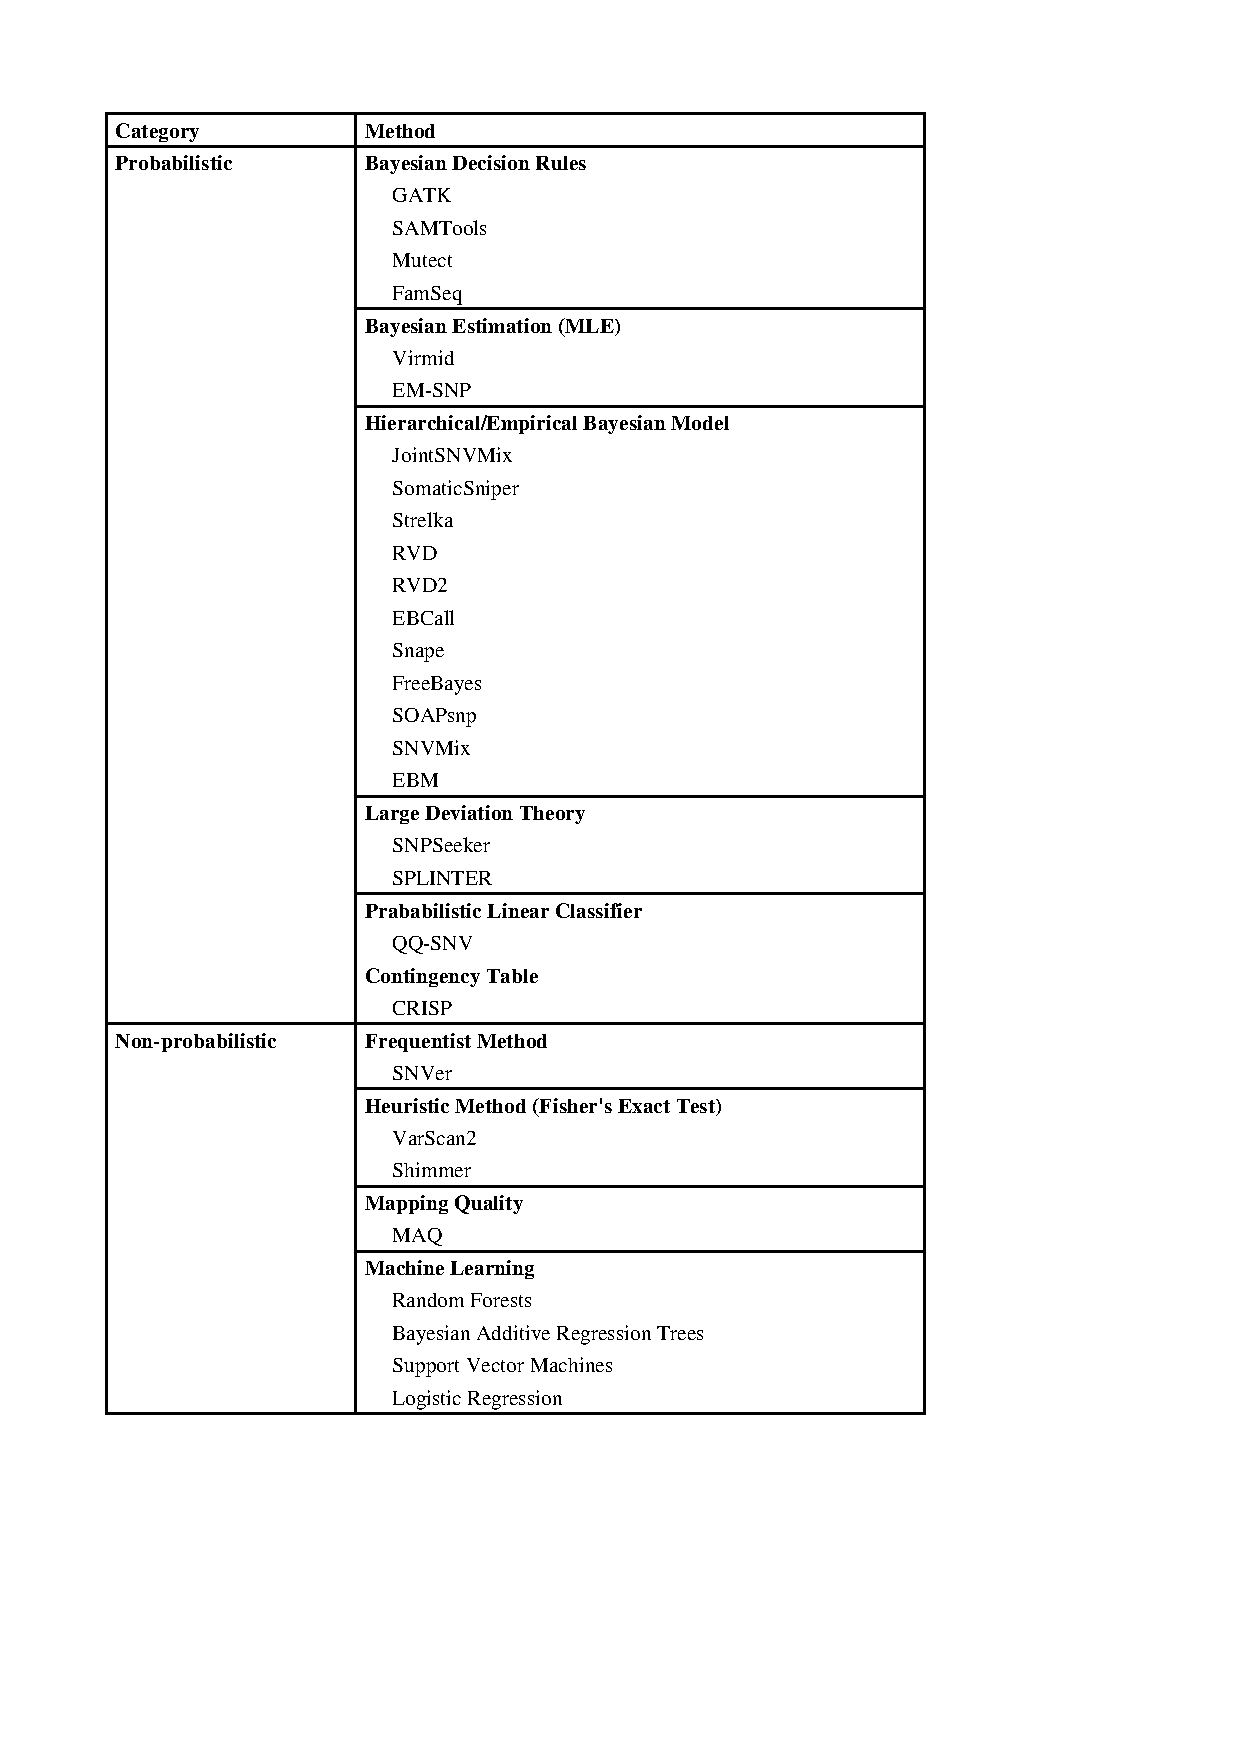
\includegraphics[width=1.2\textwidth]{method_table.pdf}
\caption{Single nucleotide variant detection methods.}
\label{tbl:methods}
\end{table}


\subsection{Probabilistic Methods}
List of 21 probabilistic methods for variant detection:

- one sentence purpose of the methods

- categories that the method falls into

- metrics and application

GATK \citep{McKenna2010},



SAMTools \citep{Li2009a},

Mutect \citep{Cibulskis2013},

FamSeq \citep{Peng2013},
Virmid \citep{Kim2013},

EM-SNP \citep{Chen2013},

JointSNVMix \citep{Roth2012},

SomaticSniper \citep{Larson2012},

Strelka \citep{Saunders2012},

RVD \citep{Flaherty2012},

RVD2 \citep{He2015},

EBCall \citep{Shiraishi2013},

Snape \citep{Raineri2012},

FreeBayes \citep{Garrison2012},

SOAPsnp \citep{Li2009},

SNVMix \citep{Goya2010},

EBM \citep{Zhou2012},

SNPSeeker \citep{Druley2009},

SPLINTER \citep{Spencer2014},

QQ-SNV \citep{VanderBorght2015},

CRISP \citep{Bansal2010}.

\subsection{Non-probabilistic Methods}
List of 8 non-probabilistic methods for variant detection:

SNVer \citep{Wei2011},

VarScan2 \citep{Koboldt2012},

Shimmer \citep{Hansen2013},

MAQ \citep{Li2008},

Random Forests \citep{Ding2012},

Bayesian Additive Regression Trees \citep{Ding2012},

Support Vector Machines \citep{Ding2012},

Logistic Regression \citep{Ding2012}.

Atlas2 \citep{challis2012integrative} uses a logistic regression model to detect SNVs that pass the heuristic filters.


\bibliography{bib}
\bibliographystyle{named}
\end{document}
